% Options: [twoside, leqno, 11pt], etc.. leqno is "number equations on the left hand side"
\documentclass[12pt]{thesis}
\usepackage{setspace}
\usepackage{amsmath}
\usepackage{graphicx}
\usepackage{wrapfig}
\usepackage{longtable}
\usepackage{subcaption}
\usepackage{setspace}
\usepackage{float}

\graphicspath{ {C:/Users/Marissa/network-similarity/} }

\usepackage{array}
\newcolumntype{L}[1]{>{\raggedright\let\newline\\\arraybackslash\hspace{0pt}\vspace{0pt}}m{#1}}
\newcolumntype{C}[1]{>{\centering\let\newline\\\arraybackslash\hspace{0pt}}m{#1}}
\newcolumntype{R}[1]{>{\raggedleft\let\newline\\\arraybackslash\hspace{0pt}\vspace{0pt}}m{#1}}

%%%%%%%%%%%%%%%%%%%%%%%%%%%%%% DOCUMENT PROPERTIES %%%%%%%%%%%%%%%%%%%%%%%%%%%%%%%%%%

\author{Marissa Graham}

% Titles must be in mixed case. Style guide: https://www.grammarcheck.net/capitalization-in-titles-101/.

\title{A Comprehensive Investigation of Graph and Network Comparison: Techniques and Applications} 

\degree{Master of Science}
\university{Brigham Young University}
\department{Department of Mathematics} 
\committeechair{Emily Evans} 

%% These are fields that are stored in the PDF but are not visible in the document itself. They are optional.
\memberA{Benjamin Webb}
\memberB{Christopher Grant}
\subject{Writing a thesis using LaTeX} % Subject of your thesis, e.g. algebraic geometry
\keywords{LaTeX, PDF, BYU, Math, Thesis}
\month{June}
\year{2018} 

\pdfbookmarks
\makeindex

%%%%%%%%%%%%%%%%%%%%%%%%% THEOREM DEFINITIONS AND CUSTOM COMMANDS %%%%%%%%%%%%%%%%%%%%%%%%%%%

%% Define the theorem styles and numbering
\theoremstyle{plain}
\newtheorem{theorem}{Theorem}[chapter]
\newtheorem{proposition}[theorem]{Proposition}
\newtheorem{conjecture}[theorem]{Conjecture}
\newtheorem{corollary}[theorem]{Corollary}
\newtheorem{lemma}[theorem]{Lemma}

\theoremstyle{definition}
\newtheorem{definition}[theorem]{Definition}
\newtheorem{example}[theorem]{Example}

\theoremstyle{remark}
\newtheorem*{remark}{Remark}

%% Create shortcut commands for various fonts and common symbols
\newcommand{\s}[1]{\mathcal{#1}}
\newcommand{\N}{\mathbb{N}}
\newcommand{\Z}{\mathbb{Z}}
\newcommand{\Q}{\mathbb{Q}}
\newcommand{\R}{\mathbb{R}}
\newcommand{\C}{\mathbb{C}}
\newcommand{\F}{\mathbb{F}}

%% Declare custom math operators
\DeclareMathOperator{\tr}{tr}
\DeclareMathOperator{\diag}{diag}
\DeclareMathOperator*{\argmin}{argmin}
\DeclareMathOperator*{\argmax}{argmax}
\DeclareMathOperator{\Span}{Span}
\DeclareMathOperator{\rank}{rank}

%% Sets and systems
\newcommand{\br}[1]{\left\langle #1 \right\rangle}
\newcommand{\paren}[1]{\left(#1\right)}
\newcommand{\sq}[1]{\left[#1\right]}
\newcommand{\set}[1]{\left\{\: #1 \:\right\}}
\newcommand{\setp}[2]{\left\{\, #1\: \middle|\: #2 \, \right\}}
\newcommand{\abs}[1]{\left| #1 \right|}
\newcommand{\norm}[1]{\left\| #1 \right\|}
\newcommand{\system}[1]{\left\{ \begin{array}{rl} #1 \end{array} \right.}

%% referencing commands
\newcommand{\thmref}[1]{Theorem \ref{#1}}
\newcommand{\corref}[1]{Corollary \ref{#1}}
\newcommand{\lemref}[1]{Lemma \ref{#1}}
\newcommand{\propref}[1]{Proposition \ref{#1}}
\newcommand{\defref}[1]{Definition \ref{#1}}
\newcommand{\exampleref}[1]{Example \ref{#1}}
\newcommand{\exerref}[1]{Exercise \ref{#1}}

\renewcommand{\labelenumi}{(\roman{enumi})}

\begin{document}








%%%%%%%%%%%%%%%%%%%%%%%%%%%%%% FRONT MATTER %%%%%%%%%%%%%%%%%%%%%%%%%%%%%%%%%%%%%%








\frontmatter 
\maketitle 

\begin{abstract}\index{abstract}
This is going to be the abstract.   
\vskip 3.25in
 
\noindent Keywords: % Keywords need to be as close to the bottom of the page as possible without moving to a new page.
\end{abstract}

%\begin{acknowledgments} \end{acknowledgments}

\tableofcontents
\listoftables
\listoffigures
\mainmatter

% REFERENCES
  % \textt{} for code font styling
  % \begin{verbatim} for printing LaTeX code as-is
  % \index{keyword} for indexing stuff
  % \cite{reference tag}
  % \section{title}, \subsection{title} (no \end thing necessary)
  % Chapter, and section show up in table of contents, subsection is bolded headings with separated paragraphs









%%%%%%%%%%%%%%%%%%%%%%%%%%%%%%%% NOTES %%%%%%%%%%%%%%%%%%%%%%%%%%%%%%%%%%%%%%%%%








Questions/Notes
\begin{itemize}
\item There's a list in the one appendix about things I think I should probably include--mostly figures
\item Commas in four digit numbers?
\item Where should the reading list network pictures go? Same place as tables, in chapter 3, or in an appendix?
%\item Provide a "not the most detailed but broad overview/guide to network similarity aka here's the main ideas and approaches and who to go read about all the specific stuff"?
\end{itemize}
Notes for me
\begin{itemize}
\item Avoid contractions
\item Fix figure references by labeling at the BOTTOM of the figure block, has to come after the caption
\item Say which python packages are used, and include a reference for non-standard ones
\item No more than one footnote every 2-3 pages.
\item No rhetorical questions outside the introduction.
\item Yes, cite CrossRef for sure.
\end{itemize}
\pagebreak








%%%%%%%%%%%%%%%%%%%%%%%%%%%%%%%% CHAPTER 1 %%%%%%%%%%%%%%%%%%%%%%%%%%%%%%%%%%%%%%%








\chapter{Introduction and Background}




\section{Motivation}

\begin{wrapfigure}{L}{0.4\textwidth}
\centering
\vspace{-20pt}
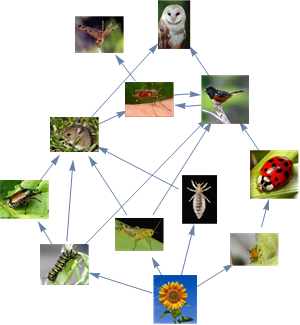
\includegraphics[width=0.38\textwidth]{foodweb.png}
\scriptsize
``SimpleFoodWeb" Mathematica sample network.
\caption{Using a network to represent relationships in a food web.}
\vspace{-20pt}
\label{fig:foodweb}
\end{wrapfigure}

Networks\footnote{The term \textit{network} is sometimes used interchangeably with the term \textit{graph}. While they both refer to the same mathematical object, we attempt to follow the heuristic throughout of using the term \textit{graph} to refer to a purely mathematical object and \textit{network} to refer to a real-world system.} are first and foremost a way to model the relationships between objects, which we do by representing objects as vertices and and relationships as edges. For example, we might use a graph to represent the relationships in a food web, or between characters in a successful movie franchise.

In some cases, using this representation simply to visualize relationships is useful, but we generally would also like to computationally exploit it in order to gain further insight about the system we are modeling. 


\begin{wrapfigure}{r}{0.5\textwidth}
\centering
\vspace{-25pt}
\includegraphics[width=0.48\textwidth,height=0.28\textwidth]{avengers.png}
\scriptsize
Diagram from the mic.com article ``Here's How the Marvel Cinematic Universe's Heroes Connect — in One Surprising Map".
\caption{Using a network to represent relationships between movie characters.}
\vspace{-20pt}
\label{fig:avengers}
\end{wrapfigure}

As a first example, consider what questions we might ask about an infrastructure network such as a road network, phone lines, power grid, or the routers and fiber optic connections of the Internet itself. How do we efficiently get from here to there? How much traffic can flow through the network? What happens if an intersection is clogged, or a power plant fails? 


We can also ask questions about social networks representing relationships between people. Who is the most important? Who controls the flow of information? To what extent do the people you consider your friends consider themselves \textit{your} friend?  How similar are you to your friends? To what extent are your friends friends with each other? How well is everybody connected to each other? To what extent do people form relationships with people who are like them? What do communities and strong friend groups look like, mathematically?

One common question across all of mathematics is how similar objects are to each other. With networks, we can ask this question about individual vertices in a network, but we also frequently want to ask it about networks themselves. For example, we might ask ``How similar are you to other students, based on your friendships at school?", but we can also ask "Which proteins, protein interactions and groups of interactions are likely to have equivalent functions across species?" %(NOTE: cite ``Modeling cellular machinery through biological network comparison", it's their exact sentence.)

For objects as combinatorially complex as networks, similarity calculation is a difficult problem, the study of which has its roots in the 60s and 70s (cite fifty years, this is almost their sentence) and, as illustrated in Figure \ref{fig:year_distributions}, has gained significant attention in the past twenty years as interesting network data becomes more readily available and computationally feasible.

The goal of this project is to provide a broad outline of the field of network similarity, but without prior expertise or expert guidance, it is laborious at best and impossible at worst to know which works are important and which are irrelevant. Instead, we use the tools of network theory to study the network of citations between scientific papers on a certain topic. This allows us to use standard network analysis techniques to determine which papers are the most important or influential, and has the additional advantage of bringing transparency to the process. That is, we can quantitatively justify our assertions using standard centrality and community detection measures, rather than relying on existing expertise in the field to give weight to our claims.

\begin{figure}[h!]
\centering
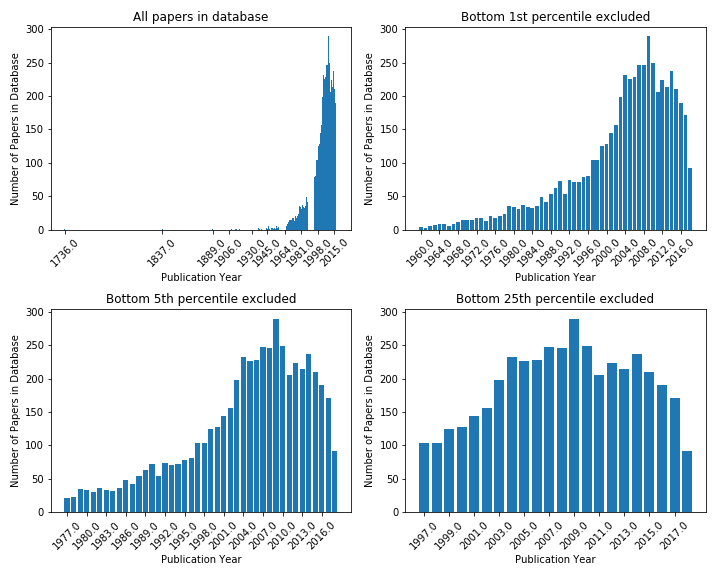
\includegraphics[width=0.9\textwidth]{year_distribution.png}
\caption{Distribution of papers published by year in our citation network of network similarity-related papers. Interestingly, year cutoffs for significant percentiles seem to roughly correspond to the spread of computers, personal computers, and the Internet, respectively.}
\label{fig:year_distributions}
\end{figure}








\section{Basic Network Properties}

\begin{figure}[h]
\centering
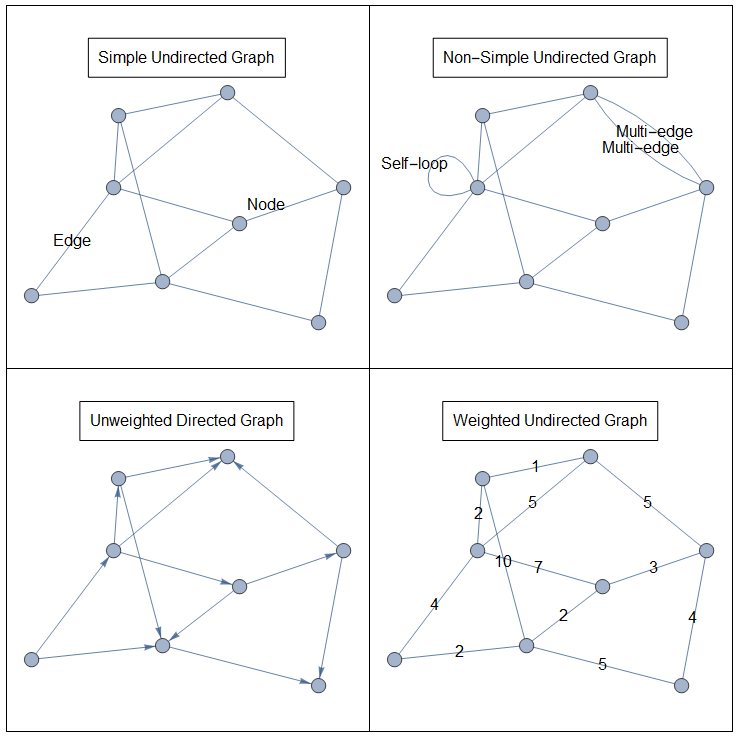
\includegraphics[width=0.9\textwidth]{basic_properties_demo.png}
\caption{Basic types of networks}
\label{fig:basic_properties_demo}
\end{figure}

In this section we introduce the definitions and notation required to give context to our analysis of the citation network. Our presentation follows Newman's \textit{Networks: An Introduction} closely, with the remainder of definitions not otherwise cited sourced from \textit{Algorithms and Models for Network Data and Link Analysis}. %cite these

A \textbf{graph}\index{graph} $G(V,E)$ is formally defined as a finite, nonempty set $V$ of \textbf{nodes}\index{nodes} or \textbf{vertices}\index{vertices}, combined with a set $E\subset V\times V$ of \textbf{edges}\index{edges} representing relationships between pairs of vertices. Throughout this work, we denote the number of vertices in a graph by $n$ and the number of edges by $m$ where not otherwise specified.

In this work we will deal with \textbf{simple graphs}\index{simple graph}, which are those that do not have more than one edge between any pair of vertices (that is, a \textbf{multiedge}\index{multiedge}), and do not have any edges from a vertex to itself (a \textbf{self-edge}\index{self-edge} or \textbf{self-loop}). 

We also are concerned with whether a graph is \textbf{directed}\index{directed graph} or \textbf{undirected}\index{undirected graph}. In an undirected graph, we have an edge \textit{between} two vertices, whereas in a directed graph we have edges \textit{from} one vertex \textit{to} another vertex. Throughout this work, we will use the notation $v_i \leftrightarrow v_j$ for an undirected edge between vertices $v_i$ and $v_j$, and $v_i \rightarrow v_j$ for a directed edge. In either case, the edge $v_i\leftrightarrow v_j$ or $v_i\rightarrow v_j$ is \textbf{incident}\index{incident} to vertices $v_i$ and $v_j$, and vertices $v_i$ and $v_j$ are therefore considered \textbf{neighbors}\index{neighbor}.

A graph can also be \textbf{weighted}\index{weighted graph}, meaning each edge is assigned some real, generally positive value $w_{ij}$ representing the ``strength" of the connection between vertices $v_i$ and $v_j$. 

In an undirected graph, the \textbf{degree}\index{degree} of a vertex is the sum of the weights of the incident edges, and in a directed graph, the \textbf{indegree}\index{indegree} and \textbf{outdegree}\index{outdegree} are the total weight of a vertex's incoming and outgoing edges, respectively. If the graph is unweighted, this is simply the number of adjacent, incoming, or outgoing edges, as the weight of each edge is one.

When studying real-world networks, we also make a distinction between \textbf{deterministic}\index{deterministic} and \textbf{random}\index{random} networks. This distinction is roughly the same as that between a variable and a random variable. The vertices and edges in a deterministic network are ``fixed", while in a random network, they need to be inferred from data using statistical inference methods. For example, our citation network is deterministic, but a network of protein interactions for a given species is not, as it must be inferred from experimental data on a limited number of members of that species.









\section{Computational Network Properties}
Whether a network is directed or weighted or simple will inform our approach to its analysis, but these properties are generally included as metadata rather than computationally determined. The remainder of the properties we consider in network analysis are determined computationally, with varying degrees of algorithmic complexity.




\subsection{Connectivity}

\begin{wrapfigure}{L}{0.3\textwidth}
\centering
\vspace{-20pt}
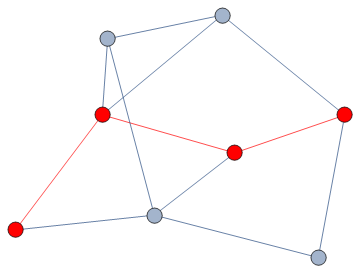
\includegraphics[width=0.28\textwidth]{path_demo.png}
\caption{A path of length three on a small network.}
\vspace{-20pt}
\label{fig:path_demo}
\end{wrapfigure}

One example of interesting computational network properties is the question of whether a network is \textbf{connected}\index{connected graph}, as illustrated in Figure \ref{fig:connectivity_demo}; that is, there is a \textbf{path}\index{path} between any pair of vertices, where a path is defined to be a sequence of vertices such that consecutive vertices are connected by an edge (link Newman? almost his sentence, but it's such a basic definition). In the case of a directed graph, we make the distinction between weak and strong connectivity. A \textbf{weakly connected graph}\index{weakly connected graph} is one which is connected when each edge is considered as undirected, while a \textbf{strongly connected graph}\index{strongly connected graph} requires a path from every vertex to every other vertex, even while respecting edge directions. 

\begin{figure}[h]
\centering
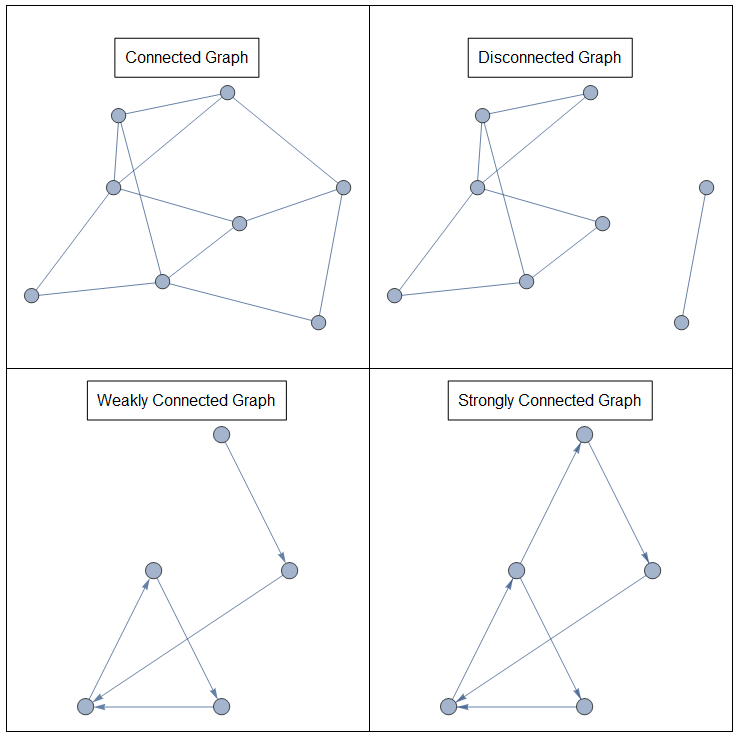
\includegraphics[width=0.9\textwidth]{connectivity_demo.png}
\caption{Simple examples of different types of network connectivity.}
\label{fig:connectivity_demo}
\end{figure}

If an undirected network is not connected, or a directed network, is not weakly connected, the network has multiple \textbf{connected components}\index{components} or \textbf{weakly connected components}. Each component is a subset of vertices such that there is a path between every pair of member vertices, and no paths between any member and a nonmember. For example, the disconnected graph in Figure \ref{fig:connectivity_demo} has two components. The weakly connected components of a directed graph are the components in the corresponding undirected network.

In a typical real world network, there is generally a single large component or weakly connected component which contains most of the vertices, with the rest of the vertices contained in many small disconnected components. We refer to this large component as the \textbf{giant component}, and its relative size gives us a measure for how ``close" a network is to being connected; the higher the percentage of vertices are in the giant component, the closer the network is to being connected.




\subsection{Assortativity}

\begin{wrapfigure}{L}{0.6\textwidth}
\centering
\vspace{-20pt}
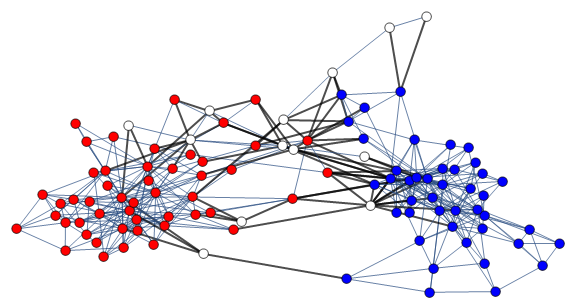
\includegraphics[width=0.58\textwidth]{assortativity_demo.png}
\scriptsize
``USPoliticsBooks" Mathematica sample network.
\caption{A network of U.S. politics books. Vertices categorized as liberal, conservative, or neutral are colored blue, red, and white, respectively, and edges that run between different categories are bolded.}
\label{fig:assortativity_demo}
\end{wrapfigure}

We can also consider whether a network is \textbf{assortative}\index{assortative}. That is, if the vertices in the network have some discrete-valued property, we ask whether the edges in the network are more likely to run between vertices of the same type. If all of the edges run between vertices of the same type, the assortativity of the network is 1; if all edges run between edges of different types, the assortativity is $-1$.

For example, the network of U.S. politics books in Figure \ref{fig:assortativity_demo} is strongly assortative with an assortativity value of $0.72$. Most of the connections are between books with the same political classification, which we can visually confirm by coloring the vertices accordingly and highlighting the few edges of the graph that run between books with different classifications.




\subsection{Acyclic networks}

\begin{figure}[h]
\centering
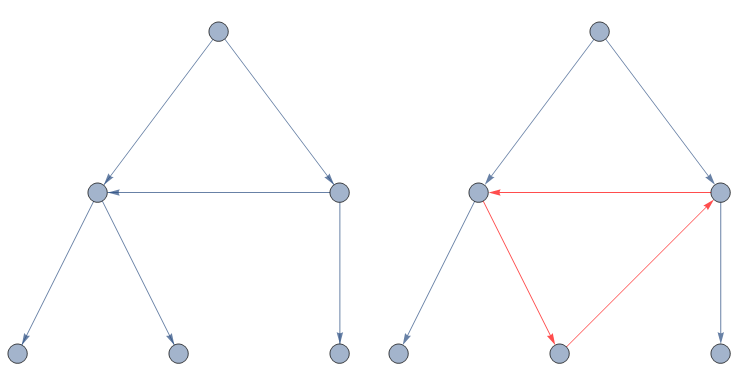
\includegraphics[width=0.58\textwidth]{acyclic_demo.png}
\caption{An acyclic directed network (left) vs. one which contains a cycle (right).}
\label{fig:acyclic_demo}
\end{figure}

We also consider whether a directed network is \textbf{acyclic}\index{directed acyclic network}, meaning that it contains no \textbf{cycles}\index{cycle} or nontrivial paths from any vertex to itself.

Our most important example of a directed acyclic network is a \textbf{citation network}\index{citation network}. In a citation network, we include an edge from a paper to each reference it cites. Any cycle in this network would require edges both from a newer paper to an older paper, and from an older paper to a newer paper. If we only cite papers which have already been written, which is the case for the papers in our dataset and generally true for academia as a whole, we cannot have any cycles. 








%%%%%%%%%%%%%%%%%%%%%%%%%%%%%%%% CHAPTER 2 %%%%%%%%%%%%%%%%%%%%%%%%%%%%%%%%%%%%%%%









\chapter{Dataset Creation and Analysis}\label{chapter:dataset_creation_and_analysis}




\section{Approach}

Citation network creation is not a trivial task. Although some journals and databases provide a citation network of the references in their own domain, when we are considering a highly interdisciplinary field, this can miss large sections of a network. As a result of this, and since intellectual property restrictions preclude simply scraping an entire citation network, we constructed the dataset manually by collecting reference lists for relevant papers and then building the network accordingly.

Relevant papers were found by searching google scholar for ``graph" or ``network" +  ``alignment", ``comparison", ``similarity", ``isomorphism", or ``matching". Topic-relevant papers were initially collected from the first five pages of results for each of the ten search terms on May 4th, 2018, after which new papers published through June 25th, 2018 were collected from a google scholar email alert for those same ten search terms. For each of these papers, we stored the plaintext reference list in a standardized format which could be easily split into the individual freeform citations. Any paper for which we have a reference list is referred to as a ``parent" record, and the references are referred to as the ``child" records. In total, we collected 7,790 child references from 221 parent papers.

In order to create the network, we needed to parse the freeform citations for each reference list to obtain metadata and recognize records as repeatedly cited. This is a difficult problem, as the records in the database span several hundred years and represent a wide variety of citation styles and languages, as well as significant optical character recognition and Unicode-related challenges. Instead of attempting to parse a citation into component parts, we used the REST API to search for each record in the CrossRef database, which already has the metadata parsed for any record it includes. We marked results as duplicate if their metadata matches and both are known to be correct, or if both their metadata and original freeform citation match exactly. 

The results given by the CrossRef API are considered correct if the title of the record can be found in the original freeform citation, and unverified otherwise. We were able to automatically verify results for about 75\% of the parent records, and about half of their children. We are conservative about marking records as duplicate, which means having so many unverified records dramatically misrepresents the structure of the network. We therefore went through the approximately three thousand unverified records by hand.

For unverified parents, we manually corrected or found title, year, author, DOI number if existent, and URL information as well as reference and citation counts. For unverified child references, we first went through and marked any correct but unverified results. We found about half of the unverified child results to be correct, despite being unable to be automatically verified due to punctuation discrepancies, misspellings, unicode issues, or citation styles that do not include the title. Next, results were counted as correct (but noted as ``half-right") if the CrossRef API returned a review, purchase listing or similar for the correct record. For the remaining incorrect references, we manually parsed the author, title, and year from the citation, or looked them up if not included. Finally, we deleted any records which did not refer to a written work of some kind; specifically, references simply citing a website, web service, database, software package/library, programming language, or ``personal communication".

We then wrote the entire citation network to a GML file which can be loaded in Mathematica. By default, the code used to generate the GML file includes the title, year, reference and citation counts for each record as vertex properties. Including further metadata as vertex properties is not difficult, but additional string-valued properties dramatically slow Mathematica's ability to load such a large network\footnote{The network contains 5,793 vertices and 7,491 edges, and takes almost exactly two minutes to load on a 2.6GHz 6th-gen quad core Intel Core i7 CPU with 16GB of RAM running Windows 10 using Mathematica 11.2.}, and a network as large as ours cannot be loaded at all, and so we do not include any more of them than strictly necessary.

The dataset itself and the code and source files used to generate it can be found on GITHUB REPOSITORY LINK, as well as documentation and instructions for using it to generate a similar dataset for any collection of properly-formatted reference list files.

\begin{figure}[p]
\centering
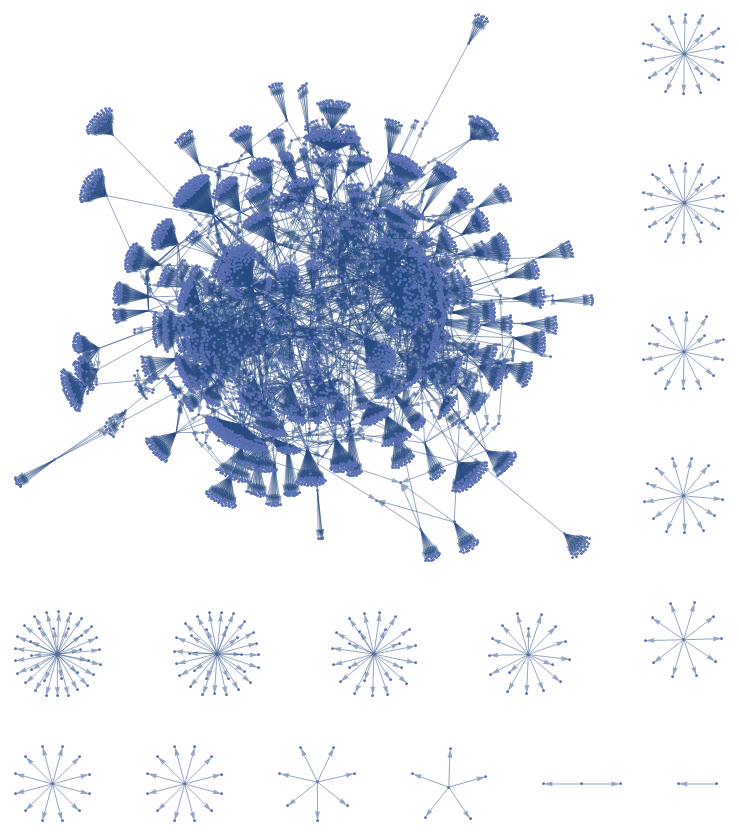
\includegraphics[width=0.9\textwidth]{full_citation_network.png}
\caption{The full citation network of the dataset used for the project.}
\label{fig:full_database}
\end{figure}








\section{Basic Statistics}


\subsubsection{Construction-related issues}

Our full citation network contains a total of 7,491 references between 5,793 papers. This results in a fairly low mean degree, or average number of references per paper, which is due to an inherent limitation in the construction of almost any citation network. We can include all the references for a small group of papers, but including all the references for \textit{their} references and so on is an exponentially more expensive task, and we therefore generally only include children for a small fraction of the total vertices. 

Since the edges in our network are hand-constructed using individual reference lists, it includes an abnormally small fraction of vertices with children. A typical citation network, such as the SciMet and Zewail datasets which are displayed in Appendix ?? and whose analysis is included in Table \ref{tab:network_table}, is constructed by scraping a single database. This results in a much higher fraction of children whose references are included, but any references which are not in the database in question are missed, so the mean degree is still quite low.

\begin{table}[h]
\centering
\begin{tabular}{|p{0.31\linewidth}||R{0.07\linewidth}|R{0.07\linewidth}|R{0.075\linewidth}|R{0.07\linewidth}|R{0.07\linewidth}|R{0.07\linewidth}|}
\hline
 & $G$ & $G_p$ & sciMet & zewail & $R$ & $R_d$ \\ \hline\hline% & $R_{d,p}$ \\ \hline\hline
Vertices & 5793 & 1062 & 1092 & 3145 & 5793 & 5793 \\ \hline % & 1077 \\ \hline %
Edges & 7491 & 2775 & 1308 & 3743 & 7491 & 7491\\ \hline % & 2775 \\ \hline
Mean degree & 1.29 & 2.61 & 1.20 & 1.19 & 1.29 & 1.29 \\ \hline %& 2.58 \\ \hline
Fraction with children & 0.038 & 0.193 & 0.523 & 0.599 & 0.733 & 0.038 \\ \hline %& 0.202\\ \hline
Diameter & 10 & 9 & 14 & 22 & 21 & 9\\ \hline % & 7 \\ \hline
Connected components & 16 & 1 & 114 & 281 & 504 & 3 \\ \hline %& 3\\ \hline
Fraction in giant component & 0.960 & 1.000 & 0.784 & 0.797 & 0.900 & 0.999 \\ \hline %& 1.000 \\ \hline
%Assortativity by indegree & 0.113 & 0.016 & 0.055 & 0.158 & 0.007 & -0.008\\ \hline % & -0.007 \\ \hline
%Assortativity by outdegree & -0.014 & -0.014 & -0.025 & 0.056 & -0.018 & -0.007 \\ \hline %& -0.013 \\ \hline
\end{tabular}
\caption{Comparing statistics for our dataset to other networks. }

\label{tab:network_table}
\end{table}


\subsubsection{The pruned network $G_p$}

\begin{figure}[h]
\centering
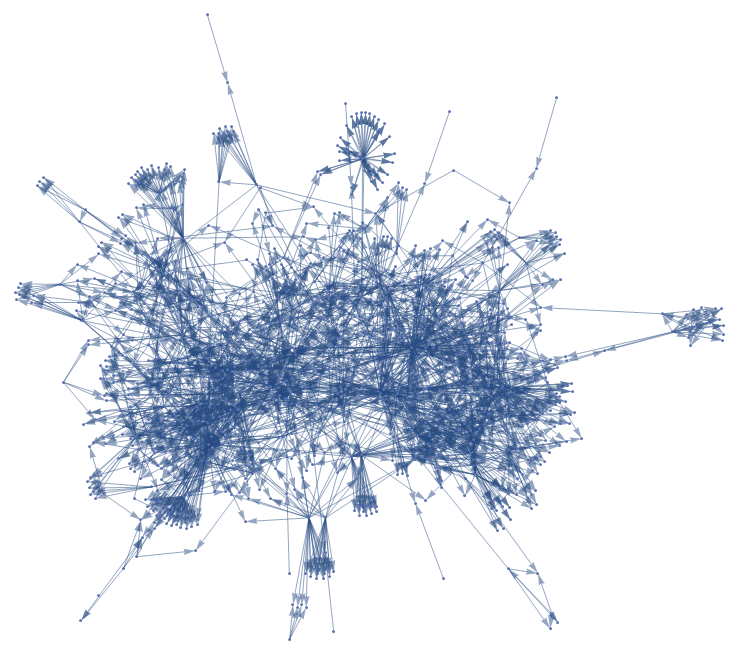
\includegraphics[width=0.9\textwidth]{subnetwork.png}
\caption{The pruned citation network.}
\label{fig:pruned_network}
\end{figure}

We also consider the \textit{pruned network}, shown in Figure \ref{fig:pruned_network}, which is defined to be the giant component of the subnetwork of vertices with positive outdegree or indegree greater than one. We do so because the main purpose of our dataset is to determine which papers are important in the field of network similarity, but the vast majority of references in the database are only cited by one paper and frequently have very little relevance to network similarity itself. 

To reduce the influence of off-topic papers on our results, we restrict our network to both our parent vertices, which we have hand-curated to be relevant to network similarity, and all vertices which are cited by more than one parent paper. This shrinks the number of vertices by a factor of almost six, correspondingly raises the fraction of vertices with children, and approximately doubles the mean degree.


\subsubsection{Comparison to other networks}
In Table \ref{tab:network_table}, we calculate the mean degree, fraction of vertices with children, diameter, number of connected components, and fraction of vertices in the giant component for six different networks: our full network $G$, its pruned version $G_p$, two datasets from the Garfield citation network collection, a uniformly generated directed random graph $R$, and a random graph $R_d$ with the same degree sequences as $G$. The random network $R$ is generated from a uniform distribution. The other, $R_d$, is constructed to match the degree sequence of $G$, by assigning each vertex ``stubs" according to the desired number of incoming and outgoing edges and then matching them by uniformly sampling the available stubs.

NOTE: DO I NEED A PICTURE FOR THIS?


\subsubsection{Connectivity}

Our full network displays a high level of connectivity; 96\% of vertices are contained in the giant component, and it has only 16 connected components, compared to 90\% containment in the giant component and 504 connected components for a randomly generated network of the same size. The diameter is also low compared to a random network and to our choices of real-world network. Since our network consists of papers collected on a specific topic, which have an outside reason to cite the same papers, this high level of connectivity is not surprising. 

The construction of the network also explains the high connectivity compared to the real-world datasets, which only have about 80\% of their vertices in their giant components; if the generation of the citation network is limited to a single database, as the sciMet and zewail datasets are, cocitation connections in other databases will be lost. This makes it more difficult for the giant component to fill the network, and results in longer paths between connected vertices.

The only dataset tested with better connectivity than ours is the random network $R_d$, which has almost complete containment--$99.9\%$--in the giant component. This is not surprising. Approximately speaking, in order for a parent vertex to be disconnected from the giant component, its children must all have exactly one parent, and no children.  In a real-world network, this is easier to find, since a paper's references are not randomly selected. A single work from an author or topic which is relatively disconnected to the rest of the network similarity academic community can generate a significant number of references which are not in the giant component. By contrast, since about $5/6$th of the vertices in $G$ have exactly one parent and no children, the probability of a parent vertex with outdegree $n$ being disconnected from the giant component is $(5/6)^n$, or $\approx 0.002$ for the average outdegree of the parents. This probability only shrinks with a higher number of disconnected parent vertices, as fewer single-parent vertices become available compared to the rest.








\section{Centrality Measures}

The main goal in creating the citation network is to determine which papers are most important or \textbf{central}\index{centrality}. The question of which vertices are the most central to a network is widely researched in network theory, and there correspondingly exists a wide variety of centrality measures used to quantify different ideas about importance. For this project, we chose five centrality measures that we expect to coincide with an intuitive definition of which papers in the network are the most relevant.


\subsubsection{Indegree} This measures the number of times each paper was cited by the parent papers in our network. Since the parent papers collectively represent everything determined to be most relevant by google scholar in a search for network comparison-related search terms, the top values for indegree should give us an idea of which papers are formative for the field and therefore more frequently cited by the parent papers.


\subsubsection{Outdegree} Since the pruned network consists of the parent papers as well as the papers that appear in more than one parent's reference list, this measures the number of a parent's references which have been cited by other parents in the network. The top values for outdegree should therefore give us an idea of which papers survey the most well-known topics in the field.


\subsubsection{Betweenness} Betweenness centrality measures the extent to which a vertex lies on paths between other vertices (sentence comes straight from newman). Intuitively, this should correspond to papers which make uncommon connections between other works; either those that are applicable to a wide variety of fields and applications, or those which build on disparate ideas in an original way. Unsurprisingly, we see some overlap between the papers with the highest outdegree and those with the highest betweenness, since the goal of a survey is to discuss a wider variety of ideas than an original paper (which only cites the specific works it builds on) can reasonably include.


\subsubsection{Closeness} 

\begin{wrapfigure}{r}{0.6\textwidth}
\centering
\vspace{-25pt}
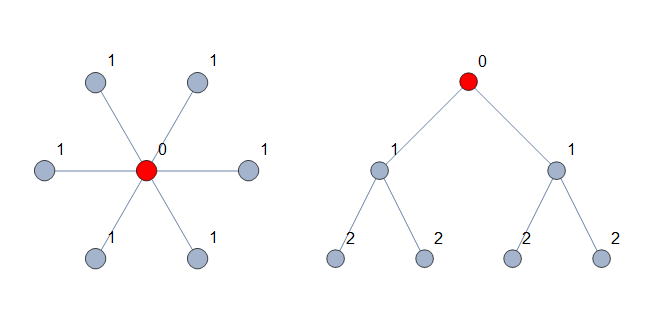
\includegraphics[width=0.55\textwidth]{closeness_demo.png}
\vspace{-10pt}
\caption{Two graphs with vertices labeled by their geodesic distance from the highlighted vertex.}
\vspace{-20pt}
\label{fig:closeness_demo}
\end{wrapfigure}

Recall that a path between two vertices is a sequence of vertices such that consecutive vertices are connected by an edge; a \textbf{geodesic path}\index{geodesic path} is the shortest possible path between any two vertices, and its length is the geodesic distance. We define \textbf{closeness} to be the inverse of the average geodesic distance between a vertex and all other vertices in the network. Closeness centrality therefore takes on the highest values for a vertex which is a short average distance from other vertices. For example, in Figure \ref{fig:closeness_demo} the highlighted vertex on the left has closeness centrality 1, since it has a distance of 1 from all other vertices. On the right, the average geodesic distance from the highlighted vertex to the other six is $\frac{1}{6}(1+1+2+2+2+2)=\frac{5}{3}$, so the closeness centrality is 0.6.

In a friendship network, this corresponds to a person who seems to either be friends with or know somebody who is friends with just about everybody. Similarly, a paper in our citation network will have higher closeness centrality if it only takes a few steps through a paper's reference list or citations to another paper's reference list or citations to get to every other paper in the network. 


\subsubsection{HITS}
For a directed network such as the citation networks used here, we may want to separately consider the notion that a vertex is important if it points to other important vertices, and the notion that a vertex is important if it is pointed to by other important vertices. This is the goal of the HITS or hyperlink-induced topic search algorithm.  We define two different types of centrality for each vertex. We have \textbf{authority centrality}\index{authority centrality}, which measures whether a specific vertex is being pointed to by vertices with high \textbf{hub centrality}\index{hub centrality}, which in turn measures whether a  specific vertex points to vertices with high authority centrality. By defining the hub and authority centralities of a vertex to be proportional to the sum of the authority and hub centralities, respectively, of its neighbors, this definition reduces to a pair of eigenvalue equations which can be easily solved numerically.








\section{High Centrality Vertices}\label{section:high_centrality_vertices}

We can observe that the pruned network, shown in Figure \ref{fig:pruned_network}, seems to contain two clusters of more tightly connected vertices.\footnote{We discuss the motivation behind and significance of this partition in detail in Chapter \ref{chapter:partitioning}.} We would like to collect the important papers for both the network as a whole and for the distinct communities it contains, so we partition the dataset in half using a modularity maximizing partition; that is, we choose two groups of vertices such that the fraction of edges running between vertices in different groups is minimized.

For both the pruned network and the two halves of our partition, we collect the top ten papers according to these five different centrality measures and summarize the results in the following tables. Since the numerical values for indegree and outdegree have intuitive meaning, we report the value itself. However, the values for betweenness, closeness, and the two HITS centralities are unintuitive, context-free real numbers, so we report the rank of each paper with respect to each measure rather than the actual value. We also calculate betweenness and closeness for the undirected version of the network, to allow those rankings to be based on citing relationships in either direction.

The papers in each table are sorted from maximum to minimum according to \[ f(p) = \frac{k^{in}_p}{k^{in}_{max}} + \frac{k^{out}_p}{ k^{out}_{max}} + \sum_{i=1}^4 \frac{1}{r_i(p)}, \] where $k^{in}_p$ and $k^{out}_p$ are the indegree and outdegree of a paper $p$, the maximums of which are taken with respect to the pruned network or partition half in question, and $r_i(p)$ is the rank of a paper $p$ according to the $i$-th of our four centrality metrics, which is defined to be infinity if a paper is not in the top ten for that metric.
 

\begin{table}[H]
\centering
\vspace{-.5cm}
{\setstretch{1}\fontsize{10.5}{13}\selectfont
\begin{tabular}{|L{0.7\linewidth}|c|c|c|c|c|c|}
\hline
Title & \rotatebox[origin=c]{90}{Indegree} &  \rotatebox[origin=c]{90}{Outdegree} & \rotatebox[origin=c]{90}{Betweenness} &  \rotatebox[origin=c]{90}{Closeness} &  \rotatebox[origin=c]{90}{HITS Auth.} & \rotatebox[origin=c]{90}{HITS Hub} \\ 
\hline\hline
*Thirty Years of Graph Matching in Pattern Recognition & 20 & 109 & 1 & 2 &  & 1 \\ \hline
$\dagger$Fifty years of graph matching, network alignment and network comparison & 6 & 71 & 2 & 1 &  & 3 \\ \hline
$\dagger$Networks for systems biology: conceptual connection of data and function & 2 & 102 & 3 & 3 &  & 2 \\ \hline
*An Algorithm for Subgraph Isomorphism & 20 & 4 & 7 & 4 & 1 &  \\ \hline
$\dagger$Modeling cellular machinery through biological network comparison & 9 & 41 & 8 &  &  &  \\ \hline
*Computers and Intractability: A Guide to the Theory of NP-Completeness & 16 & 0 & 4 & 5 &  &  \\ \hline
*The graph matching problem & 2 & 55 & 5 & 6 &  & 7 \\ \hline
$\dagger$A new graph-based method for pairwise global network alignment & 9 & 13 &  & 8 &  &  \\ \hline
$\dagger$On Graph Kernels: Hardness Results and Efficient Alternatives & 11 & 10 & 6 &  &  &  \\ \hline
*Error correcting graph matching: on the influence of the underlying cost function & 10 & 16 &  & 7 & 7 & 8 \\ \hline
*A graduated assignment algorithm for graph matching & 18 & 0 &  &  & 5 &  \\ \hline
*The Hungarian method for the assignment problem & 17 & 0 &  &  &  &  \\ \hline
*An eigendecomposition approach to weighted graph matching problems & 15 & 5 &  &  & 6 &  \\ \hline
*Recent developments in graph matching & 1 & 51 &  &  &  & 4 \\ \hline
$\dagger$MAGNA: Maximizing Accuracy in Global Network Alignment & 5 & 35 &  &  &  &  \\ \hline
*A distance measure between attributed relational graphs for pattern recognition & 14 & 0 &  &  & 3 &  \\ \hline
$\dagger$Pairwise Global Alignment of Protein Interaction Networks by Matching Neighborhood Topology & 13 & 0 &  &  &  &  \\ \hline
$\dagger$Topological network alignment uncovers biological function and phylogeny & 12 & 0 &  &  &  &  \\ \hline
A graph distance metric based on the maximal common subgraph & 10 & 0 &  & 10 & 4 &  \\ \hline
*Efficient Graph Matching Algorithms & 0 & 43 &  &  &  & 5 \\ \hline
Local graph alignment and motif search in biological networks & 8 & 10 & 10 &  &  &  \\ \hline
$\dagger$Global alignment of multiple protein interaction networks with application to functional orthology detection & 11 & 0 &  &  &  &  \\ \hline
On a relation between graph edit distance and maximum common subgraph & 11 & 0 &  &  & 2 &  \\ \hline
*Graph matching applications in pattern recognition and image processing & 0 & 40 &  &  &  & 6 \\ \hline
*Fast and Scalable Approximate Spectral Matching for Higher Order Graph Matching & 0 & 41 & 9 &  &  &  \\ \hline
*Structural matching in computer vision using probabilistic relaxation & 9 & 0 &  &  & 10 &  \\ \hline
*A new algorithm for subgraph optimal isomorphism & 2 & 21 &  &  &  & 9 \\ \hline
BIG-ALIGN: Fast Bipartite Graph Alignment & 2 & 21 &  & 9 &  &  \\ \hline
*A graph distance measure for image analysis & 8 & 0 &  &  & 8 &  \\ \hline
A new algorithm for error-tolerant subgraph isomorphism detection & 8 & 0 &  &  & 9 &  \\ \hline
*A (sub)graph isomorphism algorithm for matching large graphs & 3 & 16 &  &  &  & 10 \\ \hline
\end{tabular}
{\footnotesize$\dagger$Also top for Group 1 (biology dominated); *Also top for Group 2 (computer science dominated)}}
\vspace{-.25cm}
\caption{Highest centrality papers for the entire pruned network.}
\label{tab:toppapers_all}
\end{table}


\begin{table}[H]
{\setstretch{1}\fontsize{10.5}{13}\selectfont
\begin{tabular}{|L{0.7\linewidth}|c|c|c|c|c|c|}
\hline
Title & \rotatebox[origin=c]{90}{Indegree} &  \rotatebox[origin=c]{90}{Outdegree} & \rotatebox[origin=c]{90}{Betweenness} &  \rotatebox[origin=c]{90}{Closeness} &  \rotatebox[origin=c]{90}{HITS Auth.} & \rotatebox[origin=c]{90}{HITS Hub} \\ \hline\hline
*Networks for systems biology: conceptual connection of data and function & 2 & 90 & 1 & 2 &  & 1 \\ \hline
*Fifty years of graph matching, network alignment and network comparison & 4 & 56 & 2 & 1 &  & 2 \\ \hline
*Modeling cellular machinery through biological network comparison & 9 & 40 & 4 & 3 & 10 & 9 \\ \hline
*MAGNA: Maximizing Accuracy in Global Network Alignment & 5 & 35 & 7 & 6 &  & 3 \\ \hline
*On Graph Kernels: Hardness Results and Efficient Alternatives & 10 & 9 & 3 & 8 &  &  \\ \hline
Biological network comparison using graphlet degree distribution & 11 & 0 &  & 7 & 4 & 7 \\ \hline
*A new graph-based method for pairwise global network alignment & 8 & 12 & 9 & 4 & 6 &  \\ \hline
Network Motifs: Simple Building Blocks of Complex Networks & 11 & 0 &  & 9 & 8 &  \\ \hline
*Pairwise Global Alignment of Protein Interaction Networks by Matching Neighborhood Topology & 12 & 0 &  &  & 3 &  \\ \hline
*Topological network alignment uncovers biological function and phylogeny & 12 & 0 &  &  & 2 &  \\ \hline
NETAL: a new graph-based method for global alignment of protein-protein interaction networks & 6 & 26 &  &  &  & 5 \\ \hline
Collective dynamics of ``small-world" networks & 10 & 0 &  & 10 & 5 &  \\ \hline
Global network alignment using multiscale spectral signatures & 11 & 0 &  &  & 9 &  \\ \hline
*Global alignment of multiple protein interaction networks with application to functional orthology detection & 10 & 0 &  &  &  &  \\ \hline
Conserved patterns of protein interaction in multiple species & 10 & 0 &  &  & 7 &  \\ \hline
Pairwise Alignment of Protein Interaction Networks & 10 & 0 &  &  & 1 &  \\ \hline
Alignment-free protein interaction network comparison & 2 & 22 & 6 & 5 &  &  \\ \hline
Graphlet-based measures are suitable for biological network comparison & 1 & 30 &  &  &  & 8 \\ \hline
Survey on the Graph Alignment Problem and a Benchmark of Suitable Algorithms & 0 & 26 &  &  &  & 4 \\ \hline
Predicting Graph Categories from Structural Properties & 0 & 30 & 5 &  &  &  \\ \hline
Fast parallel algorithms for graph similarity and matching & 1 & 23 &  &  &  & 6 \\ \hline
Complex network measures of brain connectivity: Uses and interpretations & 0 & 28 & 8 &  &  &  \\ \hline
Graph-based methods for analysing networks in cell biology & 0 & 30 &  &  &  & 10 \\ \hline
Demadroid: Object Reference Graph-Based Malware Detection in Android & 0 & 25 & 10 &  &  &  \\ \hline
Early Estimation Model for 3D-Discrete Indian Sign Language Recognition Using Graph Matching & 0 & 29 &  &  &  &  \\ \hline
Indian sign language recognition using graph matching on 3D motion captured signs & 0 & 29 &  &  &  &  \\ \hline
\end{tabular}
*Also a top-centrality paper for the entire network.}
\caption{Highest centrality papers for Group 1 (biology dominated) in our partition of the pruned network.}
\label{tab:toppapers_bio}
\end{table}


\begin{table}[H]
{\setstretch{1}\fontsize{10.5}{13}\selectfont
\begin{tabular}{|L{0.7\linewidth}|c|c|c|c|c|c|}
\hline
Title & \rotatebox[origin=c]{90}{Indegree} &  \rotatebox[origin=c]{90}{Outdegree} & \rotatebox[origin=c]{90}{Betweenness} &  \rotatebox[origin=c]{90}{Closeness} &  \rotatebox[origin=c]{90}{HITS Auth.} & \rotatebox[origin=c]{90}{HITS Hub} \\ \hline\hline
*Thirty Years of Graph Matching in Pattern Recognition & 17 & 107 & 1 & 1 &  & 1 \\ \hline
*An Algorithm for Subgraph Isomorphism & 15 & 2 & 10 & 5 & 2 &  \\ \hline
*A graduated assignment algorithm for graph matching & 18 & 0 & 7 & 4 & 3 &  \\ \hline
*An eigendecomposition approach to weighted graph matching problems & 15 & 5 &  & 2 & 4 &  \\ \hline
*The graph matching problem & 2 & 36 & 3 & 3 &  & 8 \\ \hline
*A distance measure between attributed relational graphs for pattern recognition & 13 & 0 &  & 7 & 1 &  \\ \hline
*Recent developments in graph matching & 0 & 50 & 8 &  &  & 2 \\ \hline
*Error correcting graph matching: on the influence of the underlying cost function & 9 & 16 &  & 8 &  & 6 \\ \hline
*Fast and Scalable Approximate Spectral Matching for Higher Order Graph Matching & 0 & 41 & 2 &  &  &  \\ \hline
*Efficient Graph Matching Algorithms & 0 & 42 & 5 &  &  & 4 \\ \hline
*Computers and Intractability: A Guide to the Theory of NP-Completeness (Michael R. Garey and David S. Johnson) & 11 & 0 & 6 &  &  &  \\ \hline
*The Hungarian method for the assignment problem & 14 & 0 &  &  &  &  \\ \hline
*Graph matching applications in pattern recognition and image processing & 0 & 40 &  &  &  & 3 \\ \hline
Efficient Graph Similarity Search Over Large Graph Databases & 0 & 28 & 4 & 6 &  &  \\ \hline
A linear programming approach for the weighted graph matching problem & 8 & 8 &  & 9 & 9 &  \\ \hline
*Structural matching in computer vision using probabilistic relaxation & 9 & 0 &  &  & 5 &  \\ \hline
*A graph distance measure for image analysis & 8 & 0 &  &  & 6 &  \\ \hline
Inexact graph matching for structural pattern recognition & 10 & 0 &  &  &  &  \\ \hline
*A new algorithm for subgraph optimal isomorphism & 2 & 21 &  &  &  & 5 \\ \hline
Approximate graph edit distance computation by means of bipartite graph matching & 9 & 0 &  &  &  &  \\ \hline
Linear time algorithm for isomorphism of planar graphs (Preliminary Report) & 9 & 0 &  &  &  &  \\ \hline
Structural Descriptions and Inexact Matching & 9 & 0 &  &  & 7 &  \\ \hline
*A (sub)graph isomorphism algorithm for matching large graphs & 3 & 16 &  &  &  & 7 \\ \hline
A Probabilistic Approach to Spectral Graph Matching & 0 & 25 & 9 & 10 &  &  \\ \hline
Hierarchical attributed graph representation and recognition of handwritten chinese characters & 6 & 0 &  &  & 8 &  \\ \hline
Exact and approximate graph matching using random walks & 1 & 14 &  &  &  & 9 \\ \hline
A shape analysis model with applications to a character recognition system & 5 & 0 &  &  & 10 &  \\ \hline
Fast computation of Bipartite graph matching & 1 & 23 &  &  &  &  \\ \hline
Graph Matching Based on vertex Signatures & 0 & 17 &  &  &  & 10 \\ \hline
Unsupervised Domain Adaptation Using Regularized Hyper-Graph Matching & 0 & 22 &  &  &  &  \\ \hline
\end{tabular}
*Also a top-centrality paper for the entire network.}
\caption{Highest centrality papers for Group 2 (computer science dominated) in our partition of the pruned network.}
\label{tab:toppapers_CS}
\end{table}








%%%%%%%%%%%%%%%%%%%%%%%%%%%%%%%% CHAPTER 3 %%%%%%%%%%%%%%%%%%%%%%%%%%%%%%%%%%%%%%%









\chapter{Main Categories}\label{chapter:partitioning}








\section{Partitioning and Tagging the Dataset}

In the process of collecting relevant papers for our citation network, we read the abstracts for all of the parent papers, and over half the titles of their child references as we manually checked and parsed the freeform citations the CrossRef API was unable to automatically verify. While doing so, we noticed that network similarity applications seem to be almost exclusively found in the fields of biology and computer science, which we suspect should correspond to the two clusters of more densely connected vertices which we observed in Figure \ref{fig:pruned_network}.

Unfortunately, the metadata for the papers in our network does not include the subject information we would need to partition the network using on these categories; while the CrossRef API does sometimes include a ``subject" category, it is present in less than 1\% of items, and with almost six thousand references in our database, it is impractical to categorize their subjects by hand.

Instead, we partition the network into two categories of equal size, which reflects the communities we can visually observe, and set out to determine whether our two categories correspond to it in a meaningful way. 

To do so, we need some way to roughly tag papers by their subject. We chose to do according to their journal(s) of publication, since this information is available for over 97\% of the papers in our network\footnote{Journal information was not manually corrected for the papers for which the CrossRef API returned an incorrect result. However, in the vast majority of those cases, the result returned was very similar to the correct one--i.e., written by most of the same authors, or an older paper on the same subject. The subject information should therefore still be accurate enough for our purposes.}. We have a total of 2,285 unique journal names, which we tagged as ``Computer Science", ``Biology", and ``Mathematics" according to the keywords listed in Appendix ?. This allows us to reasonably quickly tag the majority of the papers as at least one of these three subjects.

Our journal-based tagging is a drastic improvement over the subject information provided by CrossRef, giving us information for about 67\% of the total papers, and 53\% of those in the pruned network. This is far from perfect, but it is enough to confirm our initial suspicions. Our goal in the remainder this chapter is to investigate how well our categories are reflected in the structure of the dataset, both overall and with respect to our partition, and then to broadly compare and contrast the study of network similarity in the fields of computer science and biology as an introduction to our discussion of each one specifically.

\begin{figure}[p]
\centering
\begin{minipage}[c]{0.23\textwidth}
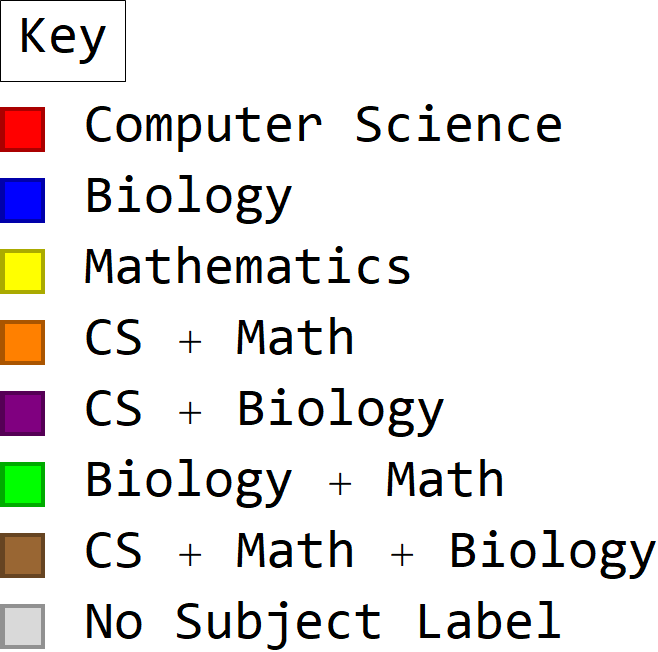
\includegraphics[width=\textwidth]{color_key.png}
\end{minipage}
\hfill
\begin{minipage}[c]{0.7\textwidth}
a)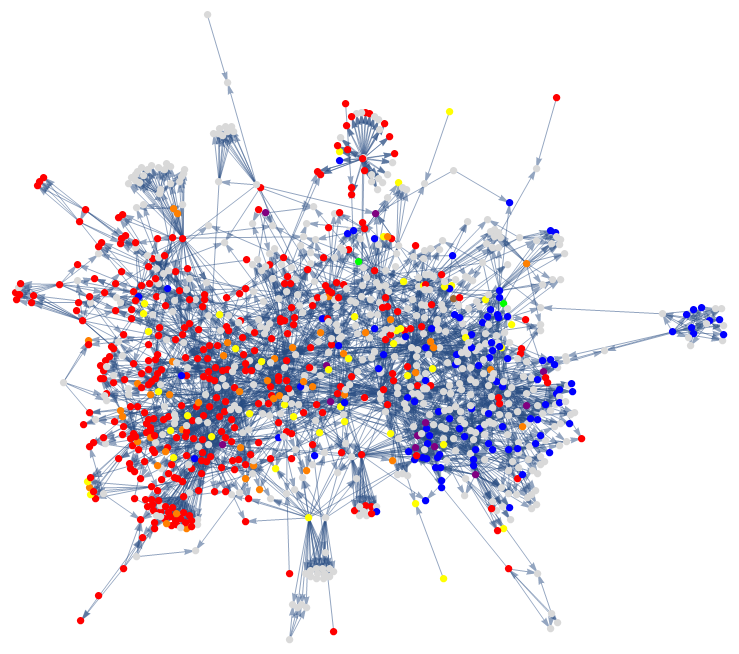
\includegraphics[width=\textwidth]{color_coded_full.png}
\end{minipage}
\begin{minipage}[c]{0.49\textwidth}
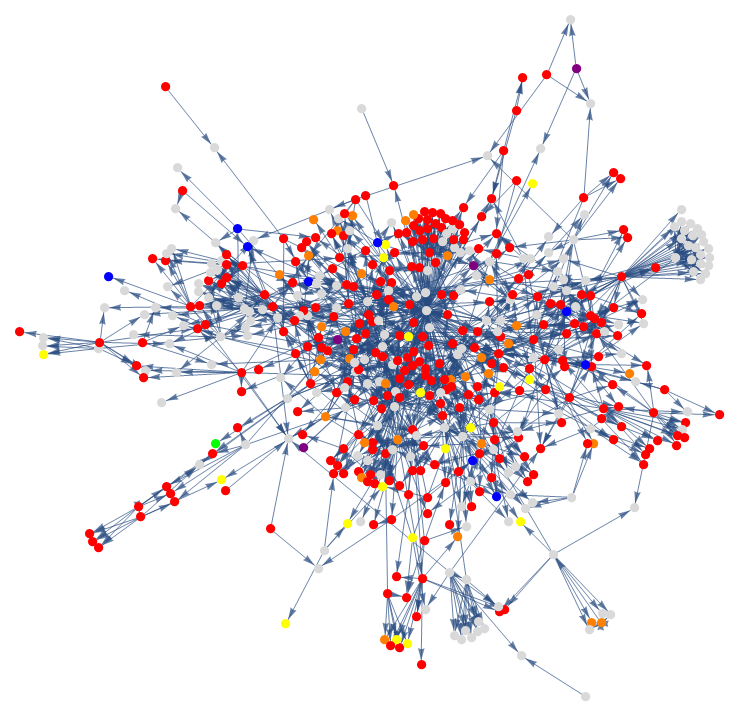
\includegraphics[width=0.95\textwidth]{color_coded_left.png}

b)
\vspace{-16pt}
\end{minipage}
\hfill
\begin{minipage}[c]{0.49\textwidth}
c)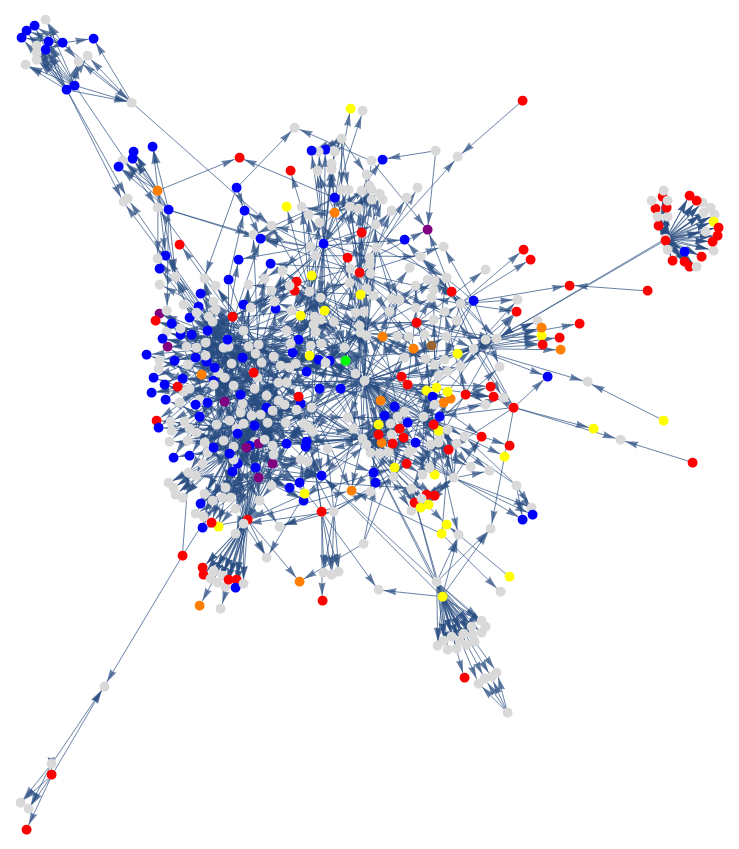
\includegraphics[width=0.95\textwidth]{color_coded_right.png}
\end{minipage}
\caption{a) The pruned network $G_p$, and b)-c) two halves of its partition $G_p^{(1)}$ and $G_p^{(2)}$, with vertices colored according to their subject label.}
\label{fig:subject_color_coded}
\end{figure}








\section{Results}








Our first step is to color code the vertices in the pruned network according to their subject, as shown in Figure \ref{fig:subject_color_coded}, so we can get a visual sense of how our tagged subjects are spread through the network. While the main two categories we are interested in are computer science and biology, we have also tagged the mathematics papers, so that we have a third category of similar size and generality as the other two. This serves as a control group, and allows us to consider and reject the hypothesis that there are three main subnetworks of similar papers instead of two. 

Intuitively, we can see that the red and blue vertices are mostly clustered together on the two halves of the pruned network, confirming our suspicion that the two dense clusters of vertices we see in Figure \ref{fig:pruned_network} correspond to the two categories we observed while constructing the dataset. We also notice that the cluster of blue vertices only fills about half of its side of the partition, indicating that the biology category is significantly smaller than the computer science category. The yellow seems to be about evenly spread across the two halves, meaning that we do not have three distinct meaningful subnetworks of papers. 

There also appear to be significantly more untagged vertices on the biology side of the partition. It is likely that this is not only because the computer science category is inherently larger, but because its papers are more likely to be tagged as such. A full half of the papers in the computer science category are published in an ACM, IEEE, or SIAM journal (IEEE journals alone represent 35\% of the CS-tagged papers), all of which are easily tagged using these acronyms as a keyword. There were not any analagous dominant organizations with acronym keywords for the biology journals in our dataset, so the tagging relies on topical keywords and therefore can identify fewer of the biology papers using a reasonable number of keywords in our search. As a result of this, the computer science network is more strongly identified as such, and therefore more structurally visible to the partitioning algorithm.

\begin{table}[t]
\centering
\begin{tabular}{|l|r|r|r|r|}
\hline & $G$ & $G_p$ & $G_p^{(1)}$ & $G_p^{(2)}$ \\ \hline
Total vertices & 5793 & 1062 & 531 & 531 \\ \hline
Untagged & 1922 & 502 & 311 & 191 \\ \hline
Tagged & 3871 & 560 & 220 & 340 \\ \hline
CS & 2533 & 405 & 93 & 312 \\ \hline
Biology & 984 & 122 & 108 & 14 \\ \hline
Math & 787 & 97 & 44 & 53 \\ \hline
Both CS and biology & 108 & 13 & 9 & 4 \\ \hline
Both CS and math & 305 & 49 & 15 & 34 \\ \hline
Both biology and math & 24 & 3 & 2 & 1 \\ \hline
All three & 4 & 1 & 1 & 0 \\ \hline
\end{tabular}
\caption{Number of vertices tagged as computer science, biology, math, or some combination of these in $G$, $G_p$, and the two halves of the partition $G_p^{(1)}$ and $G_p^{(2)}$.}
\label{tab:subject_counts}
\end{table}

We then count the number of vertices in each color-coded category, as shown in Table \ref{tab:subject_counts}. This confirms what we can intuitively see in Figure \ref{fig:subject_color_coded}. That is, almost all of the biology papers are found on one side of the partition, the majority of the computer science papers are found on the other side, and the math papers are fairly evenly spread between the two. The number of biology papers is much smaller than the number of computer science papers, which helps explain why there are more untagged papers on the biology side, and why there are significantly more computer science papers on the biology side than there are biology papers on the computer science, both by percentage and by total number.

Color codings for the full network, the subnetwork of the parent vertices, and the subnetwork of high centrality papers, as well as corresponding tables of vertex counts similar to Table \ref{tab:subject_counts}, can be found in Appendix ?.











\subsection{Assortativity results}

\begin{table}[h]
\centering
\begin{tabular}{|l|r|r|}
\hline
 & $G$ & $G_p$ \\ \hline\hline
Outdegree & -0.0178 & -0.0141 \\ \hline
Publication year & 0.0067 & 0.0041 \\ \hline
Citation count & 0.0006 & 0.0654 \\ \hline
Reference count & 0.0193 & -0.0061 \\ \hline
Tagged with any subject & 0.1089 & -0.0094 \\ \hline
Subject & 0.1837 & 0.0712 \\ \hline
Subject is CS & 0.2624 & 0.1529 \\ \hline
Subject is biology & 0.3354 & 0.1773 \\ \hline
Subject is math & 0.0732 & 0.0164 \\ \hline
Subject is CS or biology & 0.1500 & 0.0188 \\ \hline
Subject is CS or math & 0.2458 & 0.1256 \\ \hline
Subject is biology or math & 0.1713 & 0.0414 \\ \hline
\end{tabular}
\caption{Assortativity of the full and pruned citation networks with respect to various network properties.}
\label{tab:assortativity}
\end{table}

We also calculate the assortativity of the network with respect to our subject tagging, to measure the degree to which papers on a certain topic cite other papers on the same topic. In Table \ref{tab:assortativity}, we calculate the assortativity with respect to our tagged subjects, as well as various other network properties\footnote{The biggest issue we face when calculating subject-based assortativity is that our vertices can belong to multiple categories, while the assortativity algorithm requires categories to be exclusive. To handle this, we can either define category intersections to be their own, separate category, which was the approach for the ``Subject" row in Table \ref{tab:assortativity}, or we can calculate assortativity with respect to whether a vertex is or isn't tagged as a certain subject or group of subjects, which was the approach for the rest of Table \ref{tab:assortativity}.}. For non-subject properties, our assortativity values are all very low in absolute value, meaning that vertices are neither more or less likely to cite vertices with similar outdegree, publication year, citation count, or reference counts as themselves.

We do, however notice nontrivial assortativity with respect to several our subject-based properties. The values are much lower than what we observed for the example in Figure \ref{fig:assortativity_demo}, which had an assortativity of 0.72, but this is not surprising. Many of the papers on each of our topics could not be tagged as such, so the assortativity is not as high as it likely would be with perfect subject tagging. We also would not expect to see as much assortativity in the citation network of an interdisciplinary academic research area as we would in a network of non-academic political books, especially when there is significant overlap between our categories. Survey papers in particular will lower the assortativity as they draw connections between work on a similar topic, but in different disciplines.

We first notice that the assortativity values in $G_p$ are lower than their corresponding values in all of $G$. That is, the papers with only one parent, which we have removed in $G_p$, are more likely to have the same subject tag as their parent than those cited by multiple papers. This makes sense, since (I need a sentence something about interdisciplinary or whatever, it makes sense in my head but I can't think how to phrase it). 

We then observe that there is very little assortativity with respect to whether a paper's subject is mathematics, which justifies our hypothesis that the assortativity with respect to computer science and biology is noteworthy, and not observed in any subject classification.

Finally, we note that the assortativity with respect to whether a paper is either computer science or biology, or neither, is much lower than with respect to either category on its own, and only somewhat higher than the assortativity with respect to whether a paper is tagged at all. Then the assortativity with respect to whether a paper is computer science or math is only slightly lower than with respect to computer science by itself, while the assortativity with respect to whether a paper is computer science or biology is much lower than with respect to biology by itself. That is, the math category is more highly structurally linked to computer science than biology (which is unsurprising, given the relative sizes of its intersections with each category), and biology is the most structurally distinct category overall. 








\section{Preliminary category discussion}

NOT READY YET NEEDS MORE READING

Goal: Introduce the reading list subnetwork, and compare/contrast history, problem types, and methods for CS and bio

Instead of tagging the reading list network, which I should name, we printed it out big enough that you could read the titles and see for yourself, and color coded it by which side of the partition they're in. Just like the big one, you can kinda see that the bio is all in the one side of the partition, with a little bit of CS mixed in (because CS is bigger), and then the other side is all CS.



%Introduce the reading list network more, at least enough to justify inclusion of the pictures. Explain why it's so helpful to have that subnetwork, and the thing in general, while you're reading. The context is awesome. Then compare and contrast the CS vs bio. Deterministic vs random is actually the CS vs bio. What types of problems are we solving? More important quesiton might be what do the networks involved look like?

%This is one where you want to have papers in front of you to write it.

\begin{figure}[h]
\centering
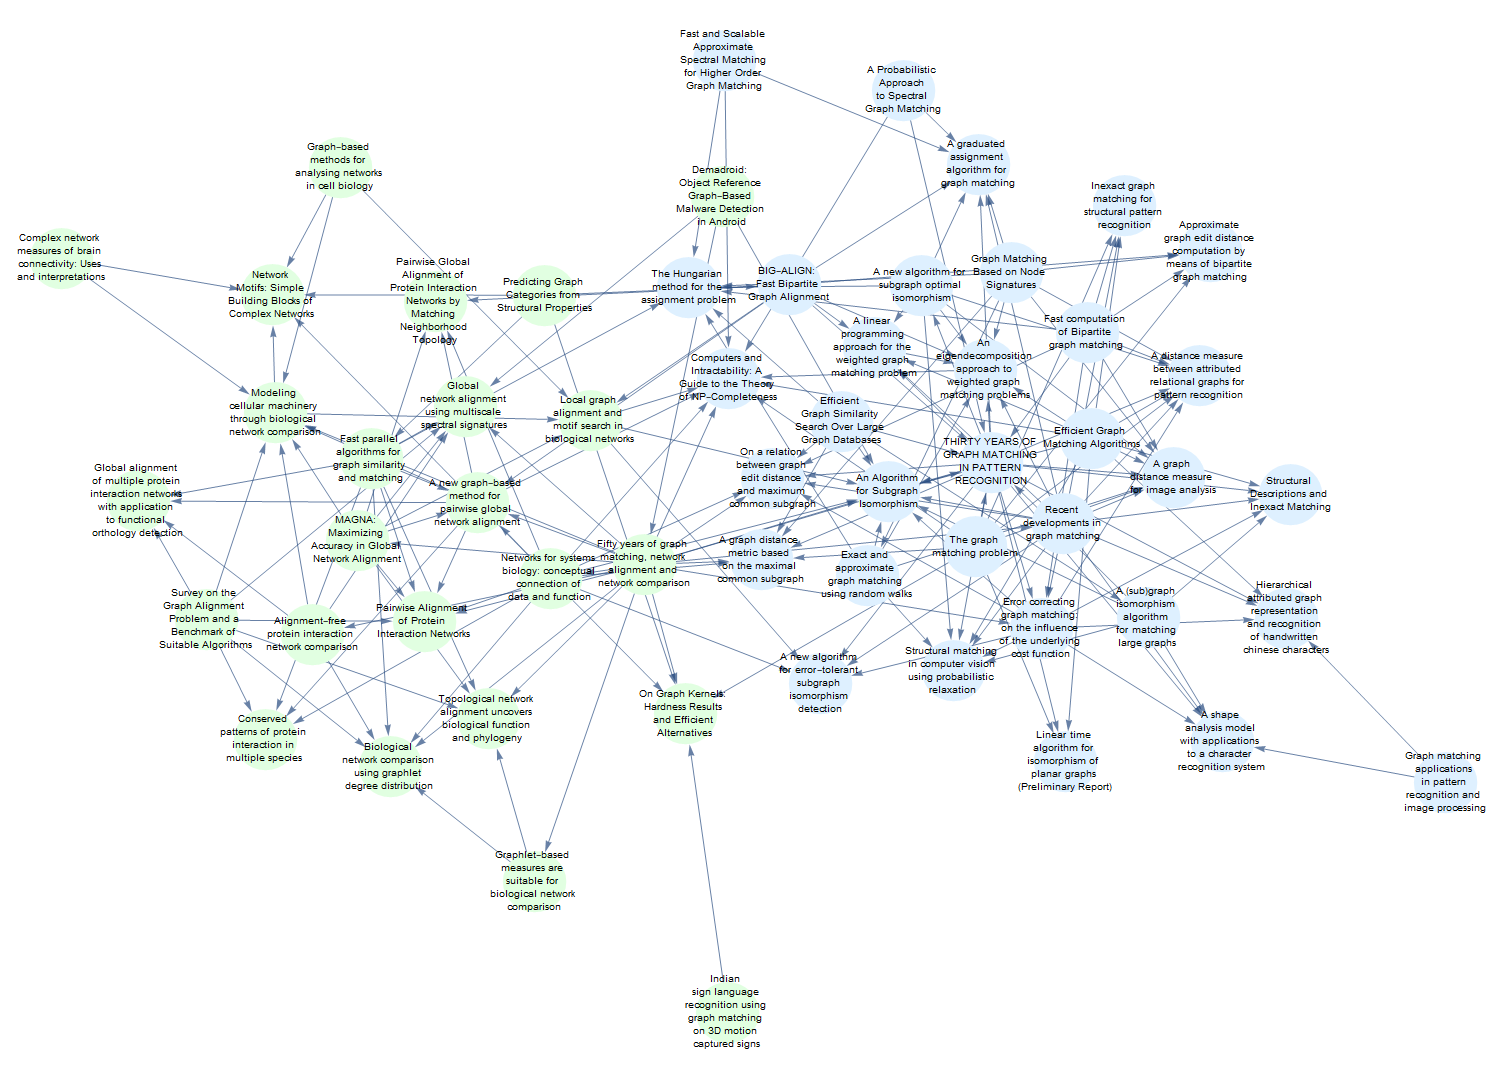
\includegraphics[width=\textwidth]{reading_list0pt9crop.png}
\caption{The subnetwork $S$ of high centrality papers, as listed in Tables \ref{tab:toppapers_all}, \ref{tab:toppapers_bio}, and \ref{tab:toppapers_CS}. Green vertices are in group 1 (biology dominated) of the partition of $G_p$, and blue vertices are in group 2 (CS dominated).}
\vspace{-12pt}\flushleft\scriptsize Note: ``Unsupervised Domain Adaptation Using Regularized Hyper-Graph Matching" is not in the connected component and is not displayed.
\label{fig:reading_list}
\end{figure}


\begin{figure}[h]
\centering
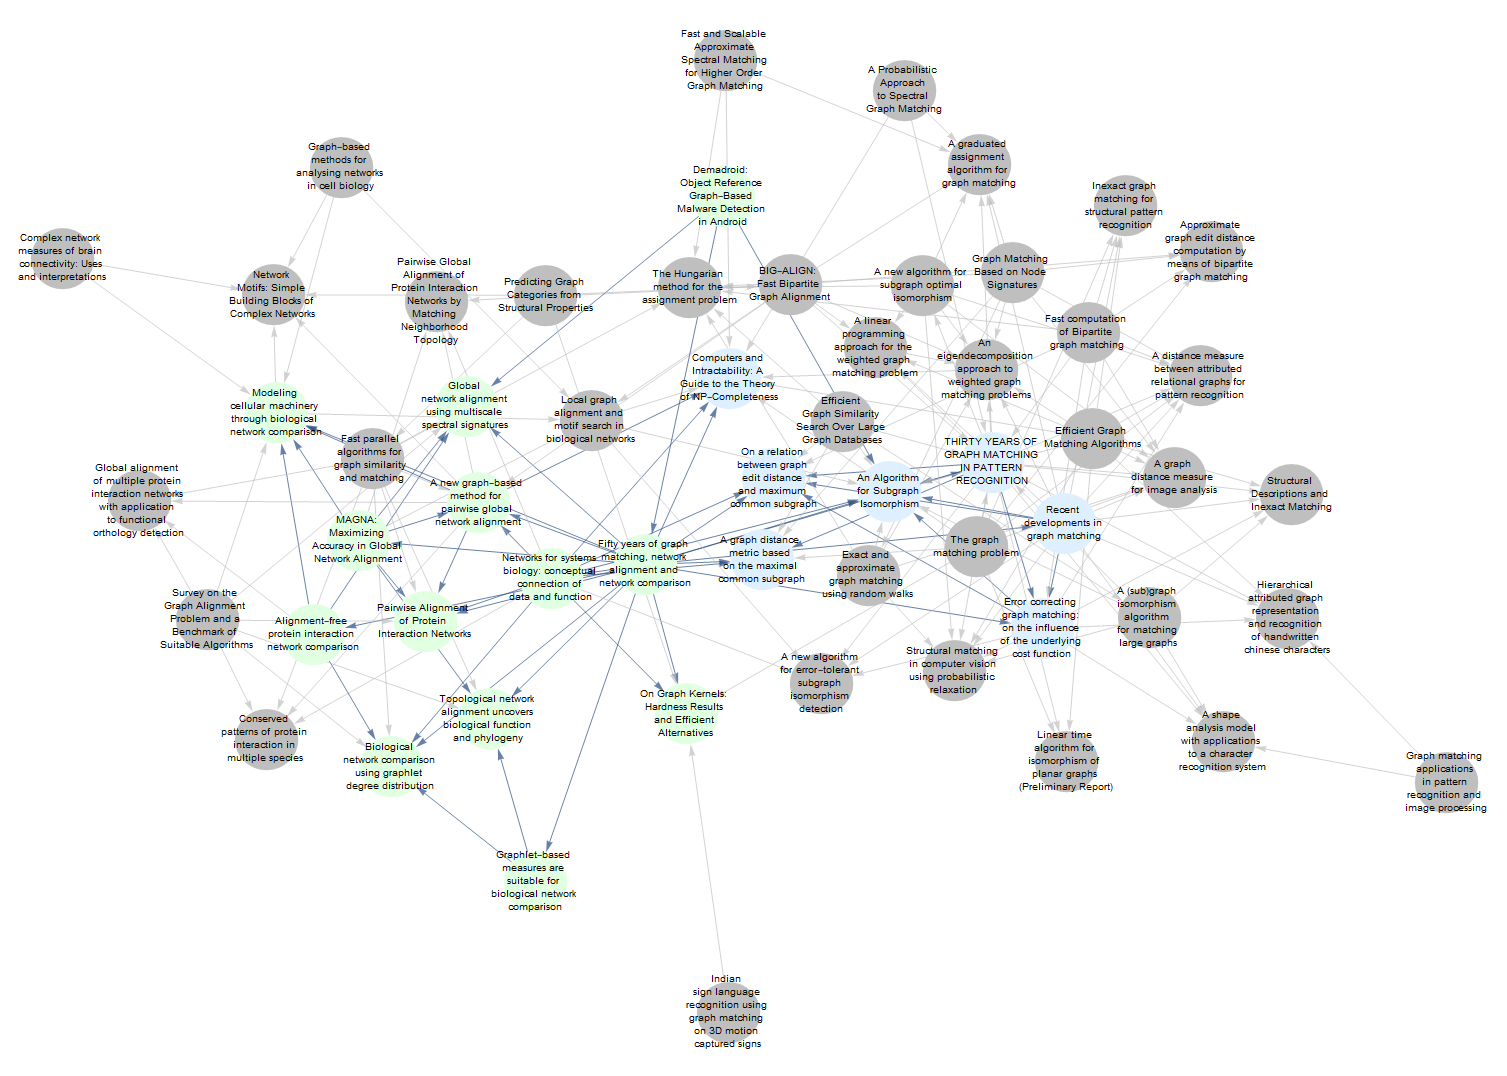
\includegraphics[width=\textwidth]{reading_list_neighborhood0pt9crop.png}
\caption{The subnetwork $S$ of high centrality vertices, highlighting the neighborhood of ``Fifty years of graph matching, network alignment, and network comparison".}
\vspace{-12pt}\flushleft\scriptsize Note: ``Unsupervised Domain Adaptation Using Regularized Hyper-Graph Matching" is not in the connected component and is not displayed.
\label{fig:reading_list_neighborhood}
\end{figure}








%%%%%%%%%%%%%%%%%%%%%%%%%%%%%%%% CHAPTER 4 %%%%%%%%%%%%%%%%%%%%%%%%%%%%%%%%%%%%%%%








\chapter{Computer Science}
 







\section{Outline and history}

2-3 pages. History of it as a field, without just doing a compare and contrast of the CS vs bio. It's mostly graph matching, because they're small and stuff.

\section{Something edit distance based}

\section{Something optimization--continuous or linear/quadratic programming?}

\section{Current shape of field, main limitations, conclusion, future work?}








%%%%%%%%%%%%%%%%%%%%%%%%%%%%%%%% CHAPTER 5 %%%%%%%%%%%%%%%%%%%%%%%%%%%%%%%%%%%%%%%








\chapter{Biology}
 







\section{Outline and history}

2-3 pages. History of it as a field, without just doing a compare and contrast of the CS vs bio. It's mostly alignment, because big and nondeterministic.

\section{Node similarity and weight matching-based alignment}

\section{Motifs and graphlet stuff}

\section{Current shape of field, main limitations, conclusion, future work?}








%%%%%%%%%%%%%%%%%%%%%%%%%%%%%%%% CHAPTER 6 %%%%%%%%%%%%%%%%%%%%%%%%%%%%%%%%%%%%%%%








\chapter{Conclusion}
 







%%%%%%%%%%%%%%%%%%%%%%%%%%%%%%%%%%% NOTES %%%%%%%%%%%%%%%%%%%%%%%%%%%%%%%%%%%%%%








\chapter{DON'T BOTHER READING THIS ONE JUST SKIP TO THE APPENDICES}



 
\subsection{Subject tagging}

Ok we already said it, but like, all the titles, I had to read ALL THE TITLES in the process of making it. All the parent titles, all the process of making the reference list text files, so many of the others, all the ones that crossref didn't get right. I am so very familiar with the titles it's not even funny. It's math in general, but the two applications and fields or people or whatever who actually use it are basically CS people and bio people. Nobody else REALLY seems to care about network similarity. You can kinda see the split into two groups once you make the partition network.

I would have done this a lot earlier or been less hesitant because like there's not at all a good built in way to tag things by subject. CrossRef has a subject category but it is a dirty, dirty liar. Barely anybody has one. Like less than one percent. Just garbage. So I was kinda accepting that I couldn't tag by subject even though that was reeeeeeeeeally a problem for the partition stuff. As if saying ``hey look, the split in half follows the modularity maximizing full partition kinda" proves the point at all. So dumb. 

Turns out though that most of them have a container title thing, and it wasn't too hard to go through and tag JOURNALS by subject keyword stuff. You don't have to trust my category judgement too much, because the lists of keywords are in a nice appendix for you. So we did that, and now we're cooking with gas. You gotta overlook the limitations though. It's muddy enough to start with and also I didn't go through and manually fix journal titles, and no way in hell am I gonna go back and do that. It's probably close enough.




\subsection{Observations?}

why is bio smaller? look what we got inside of CS. It is computer vision and natural language processing. That's pretty cool. What does the intersection look like? Biometrics and stuff. Bio people like image processing too! It is cool.

CS people really like graph matching a lot. This is kinda because of the types of problems CS likes to solve with network similarity. It's like, small networks but you have a lot. Here's a couple of examples of how certain problems turn into graph matching, maybe?

Bio people I think it's like, an extension of sequence alignment, like with DNA. The specific networks you have are very hard to get and very meaningful.

Stuff from reading the survey papers and whatnot--these are roughly the differences between the two categories, so we can frame them and stuff for the rest of it. This section gonna be haaaaaaaaaard to write and I'm gonna leave it as word vomit for a while probably. 




\subsection{What kinds of problems is bio trying to solve?}

What problems are we trying to solve when we're working with metabolic networks? Why do we care about looking up proteins?  figure out what stuff does? Why do we care about protein interaction How is DNA sequence alignment network similarity? Is it just that all these microRNA papers cite those kinds of papers a lot? 

Mapping the brain to figure out what's normal and what's important and what does what? Is that really network similarity? Community detection requires a notion of similarity.

based on a quick glance through titles, bio applications seem to be protein folding (and molecular similarity? chemical structures), metabolic interaction networks (duh) gene stuff, something something microRNA (same thing?), brain networks, SOCIAL networks, protein database search (should be similar to the graph matching ones where it's trying to find an image in a large database)

Predictions: social network and metabolic network relatively similar approach? Large networks of interactions. Molecular structure on a small scale should be like graph matching? 




\subsection{What kinds of problems is CS trying to solve?}

The main two kinds of applications seem to be computer vision and natural language processing. Both of those make sense. Unique identifiers, grading, image processing, large database search, e.g. handwriting and fingerprint/facial/iris recognition

Computer vision: fingerprint classification (lots of those, especially older ones), shape matching, pulling objects from an image, 

Natural language processing: semantic relations, obviously

Niche things: malware classification. 

Predictions and expectations for how it'll go: I think the CS stuff is pretty much exclusively graph matching. The standard techniques would be good to get from the thirty years paper, which is definitely on the list. 




\subsection{Types of problems we're trying to use network similarity for}

\begin{itemize}
\item Searching for things in a large database of small graphs (fingerprint classification, protein search, facial recognition). Nearest neighbor type thing. Unique identifiers is really more of a vertex similarity thing, but oh well.
\item Classify things as normal or anomalous (malware, cancer, trajectories, grammar, )
\end{itemize}




\subsection{Overall strategy}

\begin{itemize}
\item Very broad, intuitive overview of what this field is, why it's useful, and just the shape of it
\item Guide on how and where to get detail
\item Step through a few specific examples (ideally seminal?) to make it easier to get the idea
\end{itemize}

Guide for detail:
\begin{itemize}
\item Take a non-survey, non-seminal paper's description on the thing I want to cover
\item Condense it down to 2-3 pages, assuming a 643 level of background
\end{itemize}

What have I discovered?
\begin{itemize}
\item Seriously, the context is SO HELPFUL when you're reading!!!! I have the best context. Why is this paper considered important? Who else is citing it?
\item You find the best survey papers real easy this way (and by easy, I mean, the opposite of easy)
\item Contextualize why things are important 
\item Like, I can go look at the references and see who else also cited that, and stuff. Or like, nobody else did, so they're talking about it like it's important but maybe it isn't.
\end{itemize}




\subsection{Miscellaneous}

Explain structural assortativity. YOU STOLE THESE SENTENCES FROM WIKIPEDIA: ``The basic structure of a network can cause these measures to show disassortativity, which is not representative of any underlying assortative or disassortative mixing. Special caution must be taken to avoid this structural disassortativity."








%%%%%%%%%%%%%%%%%%%%%%%%% GLOSSARY, APPENDIX AND END MATTER %%%%%%%%%%%%%%%%%%%%%%%%%%%%%%%%








\chapter{Glossary (All background beyond the very basics for the introduction)}
We used inline definitions in the background and notations section, but we will use formal ones here.
\cite{Nobody06}

You're not going to have the black or red books in the paper list but you still need to have them in your bibliography, don't forget.

Papers go in the bibliography if you read them to put them in the chapter. Any of the ones you've got printed out, so definitely fifty years. Not all the parents need to go in the bibliography, though. You need to cite/acknowledge CrossRef, for sure. What about python packages like gspread? Idk.








% Changes the numbering of chapters and sections for appendices. Any chapters or sections listed here will be treated as part of the appendix
\appendix

\chapter{Appendices}




\section{Additional Citation Network Results}

\begin{itemize}
\item Full network, color coded by subject
\item Same for parent subnetwork and reading list
\item Tables of vertex counts for same
\item sciMet and zewail dataset figures
\item Mathematica code for making the networks besides $G$
\end{itemize}



\section{Subject Tagging Keywords}

\begin{table}[h]
\centering
\begin{tabular}{| l | l | l |}
\hline
\textbf{Computer Science} & \textbf{Biology} & \textbf{Mathematics} \\ \hline\hline
ACM & Biochem- & Algebra \\
Algorithm & Biocomputing & Algorithm \\
Artificial Intelligence & Bioengineering & Chaos \\
CIVR & Bioinformatic & Combinatori- \\
Computational Intelligence & Biological & Fixed Point \\
Computational Linguistics & Biology & Fractal \\
Computer & Biomedic- & Functional Analysis \\
Computer Graphics & Biosystem & Geometr- \\
Computer Science & Biotechnology & Graph \\
Computer Vision & Brain & Kernel \\
Data & Cancer & Linear Regression \\
Data Mining & Cardiology & Markov \\
Document Analysis & Cell & Mathemati- \\
Electrical Engineering & Disease & Multivariate \\
Graphics & DNA & Network \\
IEEE & Drug & Optimization \\
Image Analysis & Endocrinology & Permutation Group \\
Image Processing & Epidemiology & Probability \\
Intelligent System & Genetic & Riemann Surface \\
Internet & Genome & SIAM \\
ITiCSE & Genomic & Statistic- \\
Language Processing & Medical & Topology \\ 
Learning & Medicinal & Wavelet \\
Machine Learning & Medicine & \\
Machine Vision & Metabolic & \\
Malware & Microbiology & \\
Neural Network & Molecular & \\
Pattern Recognition & Neuro- & \\ 
Robotic & Neurobiological & \\
Scientific Computing & Pathology & \\
SIAM & Pathogen & \\
Signal Processing & Pharma- & \\
Software & Plant & \\
World Wide Web & Protein & \\
 & Proteom- & \\
 & Psych- & \\
 & Psychology & \\
 & Virology & \\
 & Virus & \\
\hline
\end{tabular}
\caption{Keywords used to tag journal names.}
\label{tab:tagging_keywords}
\end{table}

Table \ref{tab:tagging_keywords} contains the keywords used to tag journal names as computer science, biology, or mathematics. Both a term and its plural are considered a match, and hyphens indicate a word with several ending variations which were all considered to be associated with the tag. While the search process was case sensitive in order to avoid false positives for short words like ``ACM", case-insensitive duplicate words have been excluded from the table. The words ``algorithm" and ``SIAM" are considered to be both computer science and mathematics.

\bibliographystyle{plain}
\bibliography{thesisbib}

% If you want to include an index, this prints the index at this location. You must have \makeindex uncommented in the preamble
\printindex

\end{document}

